\documentclass[11pt,a4paper]{article}
\usepackage{graphicx}
\usepackage{titling}
\usepackage{pdfpages}
\begin{document}
\author{Ankur Dhoot}
\title{CS 471 HW}
\maketitle

\section*{Q1}

\paragraph*{(a)}
LWSN, ELLT, HAAS, SC, WTHR, BRNG, HEAV (PMU found from HEAV)

\paragraph*{(b)}
LWSN, ELLT, WTHR, HEAV, PMU

\paragraph*{(c)}
LWSN, ELLT, SC, HAAS, WTHR, HEAV, BRNG, REC, PMU

\paragraph*{(d)}
LWSN, ELLT, WTHR, HEAV, PMU

\paragraph*{(e)}
LWSN, ELLT, WTHR, HEAV, HAAS, PMU

\section*{Q2}
\paragraph*{(a)}
It very much depends on the structure of the graph. If solutions are fairly shallow, then BFS will likely do well as it expands all nodes at a given depth before going deeper. On the other hand, if solutions are fairly deep, then DFS will likely be better as it explores as deep as possible before rewinding and starting a new path. 

\paragraph*{(b)}
In a heuristic search, h(n) must underestimate the cost value to the goal, else it's possible that the algorithm will fail. If we always underestimate the cost, then all nodes which have path cost less than the optimal solution cost will be expanded since these are all possible nodes on the solution path. If we overestimate the cost, we might not expand a node that is actually on the solution path.

\paragraph*{(c)}
Example given on slide 50 of lecture 3. The reason a non-consistent heuristic can lead to some problems with graph heuristic search is that it may not be the case that the first time we expand a node, we have found the optimal f-cost to that node. Since graph search keeps a closed list of visited nodes, we only visit nodes once. Thus, if a node is on the optimal path to the solution, but we expand it prematurely (through a route not on the optimal path), then we won't be able to expand it when we are exploring the optimal path. If a heuristic is consistent, this guarantees us that whenever we expand a node, the optimal path to that node has been found. 

\paragraph*{(d)}
We'll prove that consistency implies admissibility by induction on the optimal path length, m. Let $N_{m}$ denote a node with optimal path length of m. Let $N_{*}$ denote the goal node. Let $h^{*}(N_{m})$ denote the cost of the optimal path for node $N_{m}$. 

Base case : m = 1

In this case, $N_{1}$ is an ancestor of the goal node. By consistency, we have h($N_{1}$) $\leq$ c($N_{1}$, $N_{*}$) + h($N_{*}$) = c($N_{1}$, $N_{*}$) = $h^{*}(N_{1})$ implying that a node with optimal path length of 1 satisfies the admissibility criteria.

Induction Step: Suppose true for all nodes with optimal path length $<$ m. 

Then, by consistency, h($N_{m+1}$) $\leq$ c($N_{m+1}$, $N_{m'}$) + h($N_{m'}$) for all successors $N_{m'}$ of $N_{m+1}$. In particular, since $N_{m+1}$ has optimal path of length m + 1, it has a successor, $N_{m}$, on the optimal path of length m. Applying the induction hypothesis, we get  h($N_{m+1}$) $\leq$ c($N_{m+1}$, $N_{m}$) + h($N_{m}$) $\leq$ c($N_{m+1}$, $N_{m}$) + $h^{*}(N_{m})$ = $h^{*}(N_{m+1})$ 

Thus, consistency implies admissibility. 

\paragraph*{(e)}
Preliminary result:

f-costs are nondecreasing along any path: For any successor n' of n, we have that f(n') = g(n') + h(n') = g(n) + c(n, n') + h(n') $\geq$ g(n) + h(n) by the consistency condition

Whenever a node n is expanded, the optimal path (in terms of f-cost) to that node has been found: Suppose not. That is f(n) $>$ $C^{*}$, the optimal path cost to node n. Then there must be a frontier node n' on the optimal path to n. Since f-costs are non-decreasing along any path and n' lies on the optimal path $\Rightarrow$ f(n') $\leq$ $C^{*}$ $<$ f(n) meaning n' would be expanded first. 

We have proved that whenever a node is expanded, the optimal f-cost to that node has been found. When we expand a goal node, the f-cost is just the true path length cost (since h = 0), meaning we have found the optimal path to a goal node. 

\section*{Q3}

\paragraph*{(a)}
We need to find assignments of diplomats to planets that satisfy the constraints given.

Domains:

$\alpha$ : \{ x, y, z\}

$\zeta$: \{x, y\}

$\gamma$: \{x, z\}

$\beta$: \{y\}

$\omega$: \{y, z\}

$\mu$ : \{y, z\}

Constraints:

$\zeta \neq \omega$

$\mu \neq \gamma$

Alldiff($\alpha$, $\beta$, $\omega$)

\paragraph*{(b)}
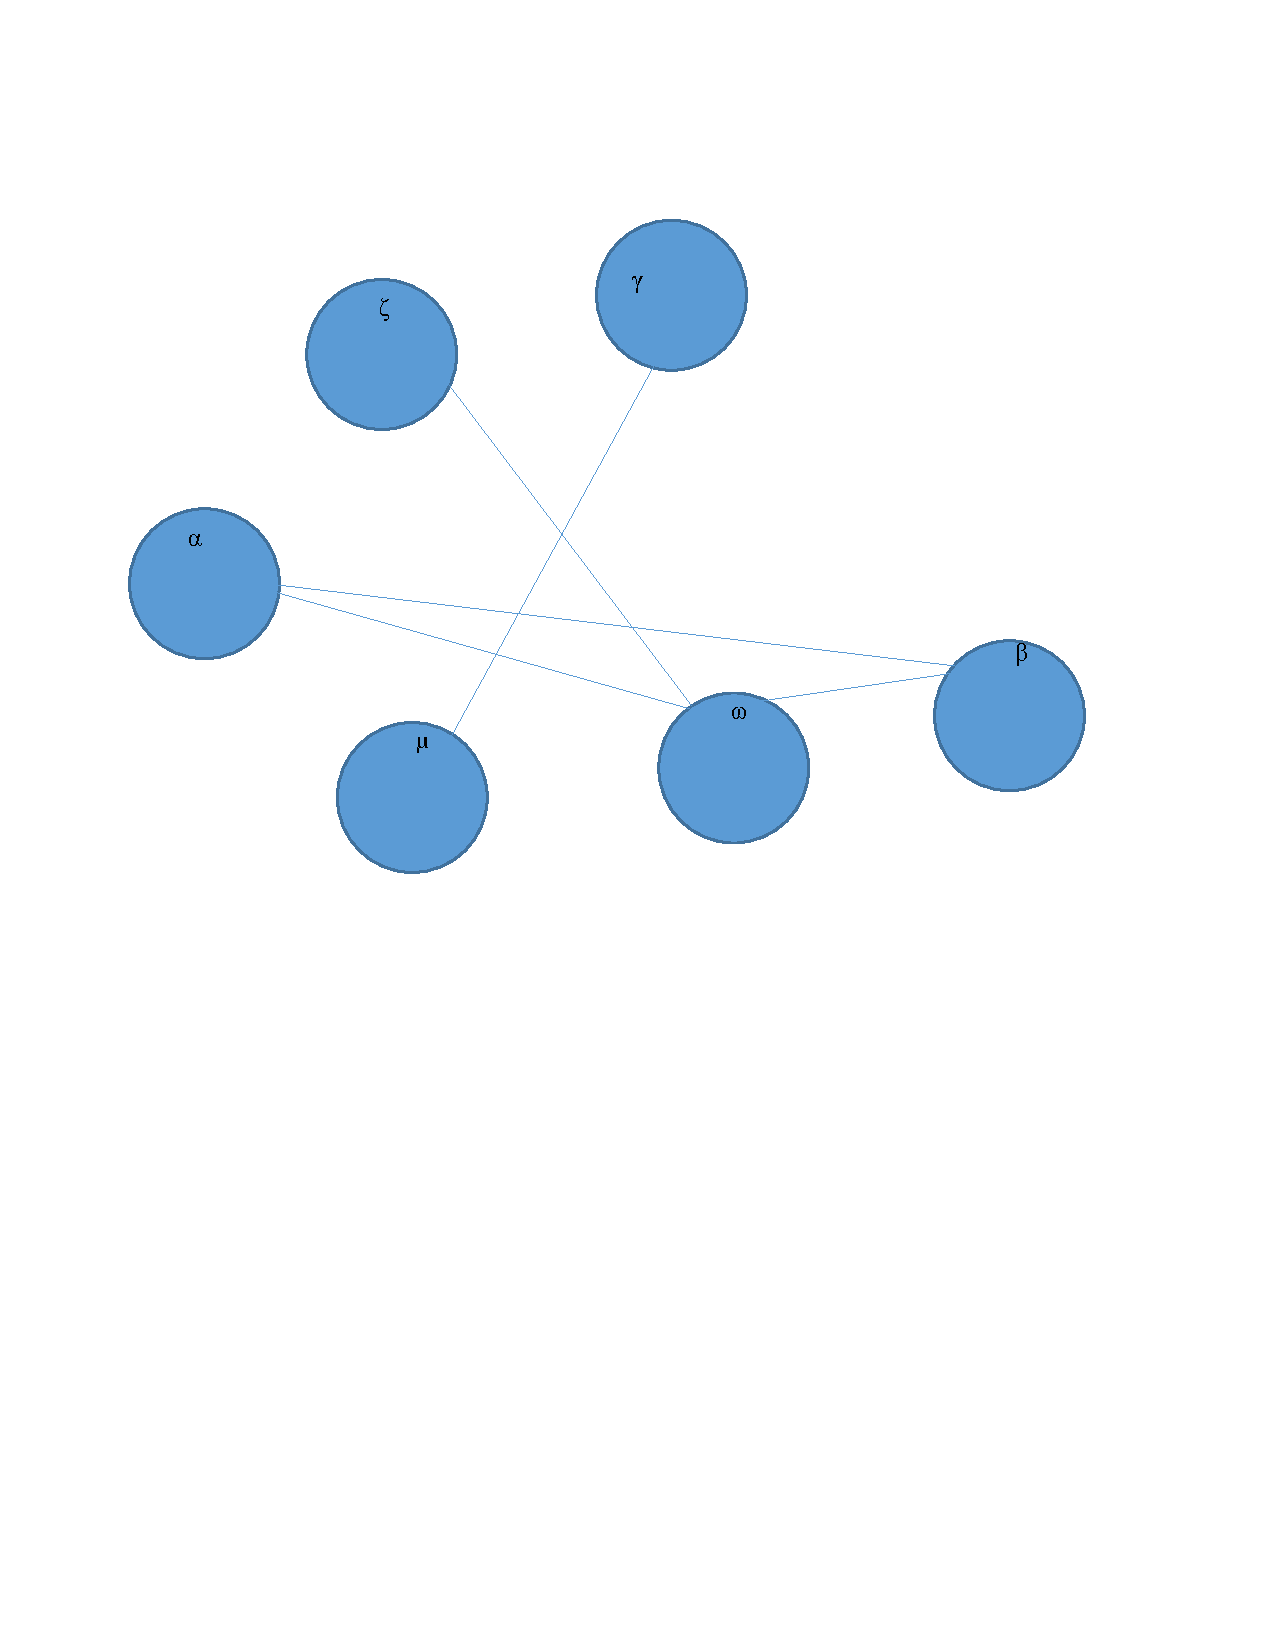
\includepdf[]{3b.pdf}


\paragraph*{(c)}

As can be seen from the constraint graph, there are two connected components, one of size 2 and one of size 4. Thus, by breaking into connected components, we can solve the problem in time O($d^{2} + d^{4}$) = O($d^{4}$).

Otherwise, if we choose a value for any of $\alpha$, $\omega$, $\beta$, then we can do a topological sort on the remaining graph (since it contains no cycles) and solve the smaller problem in O((n-1)$d^{2}$) time. 

Both of these methods are faster than checking all possible combinations which would be O($d^{6}$).

\section*{Q4}

\paragraph*{(a)}

We'll denote $R_{a}$ by A, $R_{b}$ by B, and $R_{c}$ by C.

Domains:

C1: \{A, B\}

C2: \{B, C\}

C3: \{B, C\}

C4: \{A\}

C5: \{A, C\}

C6: \{A, B\}

C7: \{B, C\}

Constraints:

C1 $\neq$ C6

C1 $\neq$ C7

C2 $\neq$ C3

C2 $\neq$ C4

C3 $\neq$ C4

C4 $\neq$ C5

\paragraph*{(b)}

The only arc that is inconsistent is C5 $\neq$ C4. Revising the domains gives C5 : \{C\}. Since there are no other arcs from C5, this is the only revision that occurs during AC-3. 

Thus, after AC-3, the domains are :

C1: \{A, B\}

C2: \{B, C\}

C3: \{B, C\}

C4: \{A\}

C5: \{C\}

C6: \{A, B\}

C7: \{B, C\}

\paragraph*{(c)}

Since C4 and C5 both have 1 remaining value, these two variables will be set first (C4 = A, C5 = C). After C4 and C5 are set, all remaining variables still have 2 remaining values. Suppose we choose C1. C1 has constraints with C6 and C7. Choosing C1 = A follows the least-constraining value heuristic (C1 = B would have reduced the domain of C6 and C7, C1 = A only reduces the domain of C6). Then, that reduces the domain of C6 to C6 : \{B\}. Thus, we then set C6 = B. C2, C3, C7 still have 2 remaining values in their domains. Suppose we choose C2. C2 has a constraint with C3. Setting C2 = B or C2 = C reduces the domain of C3 in either case by 1 so we can choose either value. Thus, we set C2 = B. That reduces the domain of C3 to C3 : \{C\}. Thus, we set C3 = 3. The last remaining variables is C7 with two values and can be set to either one. Suppose we set C7 = C.

Thus, we get C4 = A, C5 = C, C1 = A, C6 = B, C2 = B, C3 = 3, C7 = C. 
 




\end{document}
